\documentclass[tikz,border=10pt]{standalone}
% Scale from STYLE METRICS: s = 0.022663 cm per px, centred on O
\begin{document}
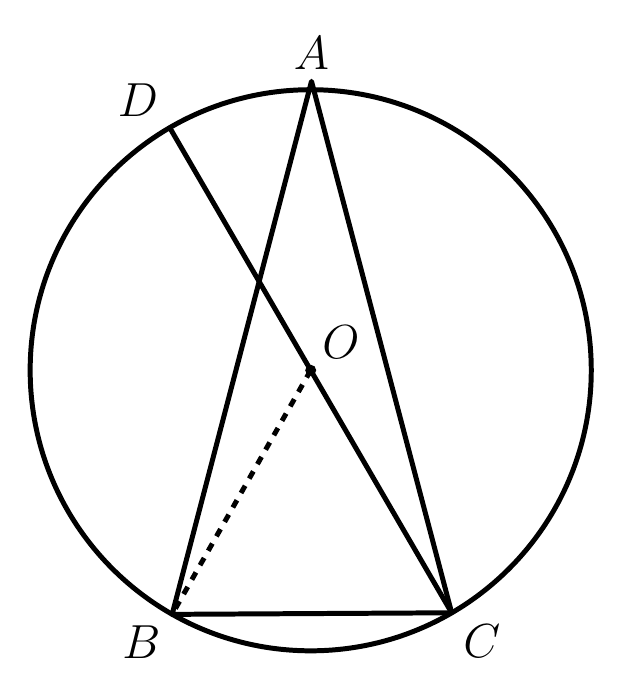
\begin{tikzpicture}[line width=1.8pt, line join=round]
  % Named coordinates (x=(px-185.6)*s, y=(222.4-py)*s)
  \coordinate (O) at (0,0);
  \coordinate (A) at (0.01,3.67);
  \coordinate (B) at (-1.76,-3.10);
  \coordinate (C) at (1.79,-3.08);
  \coordinate (D) at (-1.79,3.08);

  % Circle, radius 157.24 px
  \draw (O) circle (3.563);

  % Solid triangle ABC
  \draw (A) -- (B) -- (C) -- cycle;

  % Solid diameter DC through O
  \draw (D) -- (C);

  % Dashed radius OB
  \draw[dashed] (O) -- (B);

  % Centre dot
  \fill (O) circle (0.07);

  % Labels
  \node[font=\fontsize{19}{22.8}\selectfont, above] at (A) {$A$};
  \node[font=\fontsize{19}{22.8}\selectfont, below left] at (B) {$B$};
  \node[font=\fontsize{19}{22.8}\selectfont, below right] at (C) {$C$};
  \node[font=\fontsize{19}{22.8}\selectfont, above left] at (D) {$D$};
  \node[font=\fontsize{19}{22.8}\selectfont, above right] at (O) {$O$};
\end{tikzpicture}
\end{document}